%% LyX 1.6.5 created this file.  For more info, see http://www.lyx.org/.
%% Do not edit unless you really know what you are doing.
\documentclass[english,journal=jctcce,manuscript=article,layout=twocolumn]{achemso}
\renewcommand{\familydefault}{\rmdefault}
\usepackage[T1]{fontenc}
\usepackage[latin9]{inputenc}
\usepackage{amsthm}
\usepackage{amsmath}
\usepackage{graphicx}
\usepackage{esint}

\makeatletter

%%%%%%%%%%%%%%%%%%%%%%%%%%%%%% LyX specific LaTeX commands.
%% Because html converters don't know tabularnewline
\providecommand{\tabularnewline}{\\}

%%%%%%%%%%%%%%%%%%%%%%%%%%%%%% User specified LaTeX commands.
%%%%%%%%%%%%%%%%%%%%%%%%%%%%%%%%%%%%%%%%%%%%%%%%%%%%%%%%%%%%%%%%%%%%%
%% This is a (brief) model paper using the achemso class
%% The document class accepts keyval options, which should include
%% the target journal and optionally the macuscript tye
%%%%%%%%%%%%%%%%%%%%%%%%%%%%%%%%%%%%%%%%%%%%%%%%%%%%%%%%%%%%%%%%%%%%%


%%%%%%%%%%%%%%%%%%%%%%%%%%%%%%%%%%%%%%%%%%%%%%%%%%%%%%%%%%%%%%%%%%%%%
%% Place any additional packages needed here.  Only include packages
%% which are essential, to avoid problems later.
%%%%%%%%%%%%%%%%%%%%%%%%%%%%%%%%%%%%%%%%%%%%%%%%%%%%%%%%%%%%%%%%%%%%%
\usepackage[version=3]{mhchem}% Formula subscripts using \ce{}
%%%%%%%%%%%%%%%%%%%%%%%%%%%%%%%%%%%%%%%%%%%%%%%%%%%%%%%%%%%%%%%%%%%%%
%% If issues arise when submitting your manuscript, you may want to
%% un-comment the next line.  This provides information on the
%% version of every file you have used.
%%%%%%%%%%%%%%%%%%%%%%%%%%%%%%%%%%%%%%%%%%%%%%%%%%%%%%%%%%%%%%%%%%%%%
%%\listfiles
%%%%%%%%%%%%%%%%%%%%%%%%%%%%%%%%%%%%%%%%%%%%%%%%%%%%%%%%%%%%%%%%%%%%%
%% Place any additional macros here.  Please use \newcommand* where
%% possible, and avoid layout changing macros (which are not used
%% when typesetting).
%%%%%%%%%%%%%%%%%%%%%%%%%%%%%%%%%%%%%%%%%%%%%%%%%%%%%%%%%%%%%%%%%%%%%
\newcommand*{\mycommand}[1]{\texttt{\emph{#1}}}

%%%%%%%%%%%%%%%%%%%%%%%%%%%%%%%%%%%%%%%%%%%%%%%%%%%%%%%%%%%%%%%%%%%%%
%% Meta-data block
%% ---------------
%% Each author should be given as a separate \author command.
%%
%% Corresponding authors should have an e-mail given after the author
%% name as an \email command.
%%
%% The affiliation of authors is given after the authors; each
%% \affiliation command applies to all preceding authors not already
%% assigned an affiliation.
%%
%% The affiliation takes an option argument for the short name.  This
%% will typically be something like "University of Somewhere".
%%
%% The \altaffiliation macro should be used for new address, etc.
%%%%%%%%%%%%%%%%%%%%%%%%%%%%%%%%%%%%%%%%%%%%%%%%%%%%%%%%%%%%%%%%%%%%%
\author{Mat\'ias A. Nitsche}\affiliation{Departamento de Computaci�n FCEN-UBA}
\author{Mariano C. Gonz\'alez Lebrero}\email{mcgl@qb.ffyb.uba.ar}\affiliation{Instituto de Qu�mica y Fisicoqu�mica Biol�gicas, IQUIFIB, CONICET, ARGENTINA}

%%%%%%%%%%%%%%%%%%%%%%%%%%%%%%%%%%%%%%%%%%%%%%%%%%%%%%%%%%%%%%%%%%%%%
%% The document title should be given as usual
%% A short title can be given as a *suggestion* for running headers.
%%%%%%%%%%%%%%%%%%%%%%%%%%%%%%%%%%%%%%%%%%%%%%%%%%%%%%%%%%%%%%%%%%%%%
\title[short title?]{A GPU accelerated implementation of DFT for hybrid QM/MM simulations.}

\@ifundefined{showcaptionsetup}{}{%
 \PassOptionsToPackage{caption=false}{subfig}}
\usepackage{subfig}
\makeatother

\usepackage{babel}

\begin{document}
\begin{abstract}
This paper presents an implementation of electronic structure calculations
based on density functional theory (DFT). This development is optimized
for performing hybrid molecular dynamics simulations (QM / MM) by
making use of graphic processors (GPU) for the most computationally
demanding parts. The proposed implementation is able to make use of
modern GPUs and to achieve accelerated calculation in relevant portions
between 20 to 10 times faster than the CPU version, even in small
quantum systems. Besides, we introduce other minor optimizations that
significantly reduce the initialization time and the number of iterations
required for convergence, which is especially important in molecular
dynamics (in which thousands or millions of calculations on small
systems are performed). The presented code was extensively tested,
both in terms of numerical quality and performance over systems of
different size and composition.
\end{abstract}
\maketitle

\section{Introduction}

The simulation of chemical properties in complex systems (solution,
proteins, etc.) with electronic detail generally requires treatment
by means of computationally expensive methods. One approach is to
treat these systems using hybrid (QM/MM) methods. In this approach
the system is divided into a subsystem treated with a Hamiltonian
based on quantum mechanics while the rest is modeled with a classical
Hamiltonian. This methodology allows for the treataments of complex
systems with many degrees of freedom. However, the computational cost
associated with the resolution the self-consistent electronic problem
remains a major constraint when applying this type of model.

On the other hand, given the immense computing capabilities of the
current graphics processing units (GPU), these appear as attractive
alternatives in the area of high-performance computing. In particular,
the use of GPUs in quantum-chemistry has allowed to obtain interesting
results. There are several works that employ GPUs in diverse electronic-structure
calculations\cite{yasuda_anterior,vogt,ufimtsev,genovese2009density,hamada,gpumd,anderson},
and there's even a commercial software developed exclusively for this
kind of hardware\cite{Petachem}. A particularly relevant work is
Yasuda's\cite{yasuda2008accelerating}, in which an algorithm for
the exchange-correlation calculations related to self-consistent field
iterations (SCF) is presented. It is important to take into consideration
that the possibility of obtaining efficient algorithms depends strongly,
aside from the hardware to be used, on the type of systems that have
to be solved (size, type of atoms, basis-functions, etc.).

In our case, it is of great interest the use of hybrid simulation
techniques (QM/MM) to study bio-molecules active sites: the presented
implementation is oriented towards these systems, which usually are
not bigger than 50 or 100 atoms and which may include relatively heavy
elements such as Iron, Sulfur, Copper, etc.\cite{capece2006heme,crespo2003dft,crespo2005multiple,crespo2005theoretical,friesner2005ab,marti2004qm,ridder2003ab,sproviero2006qm}.
Molecular dynamics simulations involve performing complete DFT calculations
a large number of times, each with only a few iterations. This implies
that the initialization time has a greater relative weight in this
kind of calculation than in a single-point SCF computation.

In summary, we propose a GPU implementation oriented towards QM/MM
molecular dynamics calculations of the most computationally demanding
steps of a DFT, with Gaussian basis, calculation. This work is based
on the code Molecole\cite{molecole} and include novel approaches
having a positive impact on parallelization and performance without
affecting numerical quality. One of these differences consists in
including a new partitioning strategy for the set of quadrature points,
which results in a more efficient grouping of computational batches
in terms of performance and significative functions. Another aspect
involves using a low-cost classification criteria for determining
these significative functions, which does not require computing the
actual function values. While other implementations \cite{yasuda}
proposed the recalculation of function values several times at each
iteration, in our implementation we precompute these, obtaining notable
performance improvements. 

A CPU implementation was also developed and compared to the GPU version.
The CPU version is not simply a translation of the GPU implementation
since specific CPU features (like SSE2 instructions) were used to
obtain the best performance possible. Finally, we present and test
a hybrid code made by the coupling of our DFT implementation with
AMBER 11\cite{amber11}.


\section{Method}

In the DFT approach, the energy is written as a functional of the
density:

{\footnotesize \begin{equation}
E[\rho]=T_{s}[\rho]+V_{ne}[\rho]+\frac{1}{2}\int\int\frac{\rho(\vec{r}_{1})\rho(\vec{r}_{2})}{r_{12}}d\vec{r_{1}}d\vec{r}_{2}+E_{xc}[\rho]\label{eq:DFT}\end{equation}
}{\footnotesize \par}

where the first term is the kinetic energy associated with the density,
the second is the interaction between the density and the nuclei,
the third one is the Coulombs repulsion of the density with itself
and the last is the exchange and correlation energy\cite{kohnsham}.

The global exchange-correlation portion is the most expensive in terms
of computational cost. The energy corresponding is calculated by the
integral of the local exchange-correlation energy as: \begin{equation}
E_{XC}=\int\rho(r)\epsilon_{xc}(\rho(r))dr\label{xc}\end{equation}
 Equation {[}\ref{xc}{]} can be computed as a discrete sum over a
grid\cite{becke}: \begin{equation}
E_{XC}\cong\sum_{j}\rho(r_{j})\epsilon_{xc}(\rho(r_{j}))\label{sum}\end{equation}
 where the density $\rho$ (and its gradient, for GGA functionals)
over each grid point $j$ is calculated from the molecular orbitals
$\psi_{i}$ as: \begin{equation}
\rho(r_{j})=\sum_{i}|\psi_{i}(r_{j})|^{2}\label{rho}\end{equation}
 with \begin{equation}
\psi_{i}(x,y,z)=\sum_{k=1}^{n}c_{i}^{k}\chi_{k}\end{equation}
 where $c_{i}$ are the variational coefficients, and the orbitals
$\psi_{i}$ are constructed by expanding them in a basis of contracted
Cartesian Gaussian functions as: \begin{equation}
\chi_{k}=(x-x_{0})^{n_{x}^{k}}(y-y_{0})^{n_{y}^{k}}(z-z_{0})^{n_{z}^{k}}\sum_{j}k_{j}^{k}e^{-\alpha_{j}(\vec{r}-\vec{r_{0}})^{2}}\end{equation}
 where \begin{equation}
(\vec{r}-\vec{r_{0}})^{2}=(x-x_{0})^{2}+(y-y_{0})^{2}+(z-z_{0})^{2}\end{equation}


The computation of the exchange and correlation energy (and the corresponding
Khon-Sham matrix elements) involves several distinct steps, for all
of which a linear-scaling algorithm exists. Still, all steps exhibit
a degree of parallelism inherent to their mathematical formulation.
Exploiting this aspect gives a great advantage over serial calculations.
Nevertheless, there is not a definitive parallel implementation known
a priory since the computation can be approached in different ways.
One possible solution consists in parallelizing these steps independently
and determining the most adequate parallelization strategy for each
case. The main computational steps are: (a) quadrature-point positions
and weights, (b) function values, (c) density at each point and (d)
Kohn-Sham matrix elements. 

To achieve a linear-scaling implementation, Stratman et al propose
several strategies\cite{Stratmann1996213}. As a whole, the main idea
consists in grouping quadrature-points instead of solving the computation
for each one. This grouping permits determining which basis-functions
have a signification contribution to the final computation, which
are referred to as \emph{significative functions}. Given the rapid-decay
of Gaussian functions, the size of the set of significative functions
associated with each group of quadrature points does not depend on
the number of atoms. In other words, this size is of constant order
in terms of computational complexity. As a consequence, it is possible
to sub-divide the complete DFT calculation by computing each of these
groups independently. 


\subsection{The grid}

An important aspect of the calculation is the shape of the grid on
which Equation \ref{sum} is applied. The usual practice is to generate
a grid for the molecule via atomic overlapping grids. These atomic
grids come from the superposition of layers derived by scaling a reference
layer (see \ref{Flo:grilla}).

%
\begin{figure}
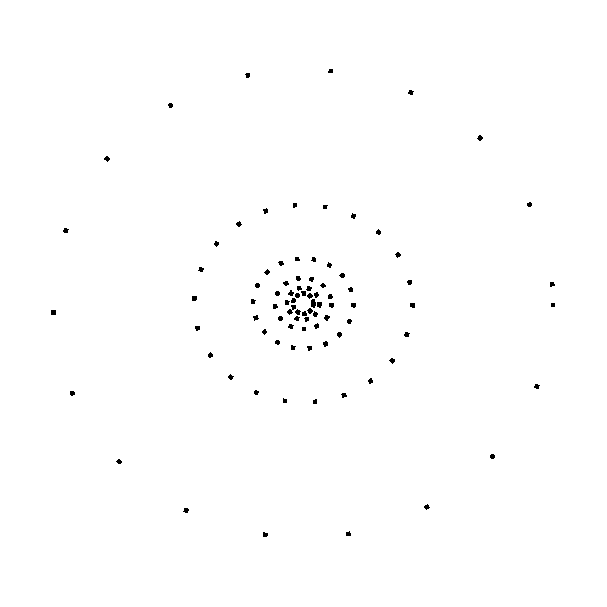
\includegraphics[scale=0.5]{figuras/grilla}\caption{Schematic atomic grid}


\label{Flo:grilla}


\end{figure}


These layers are not equidistant but are most concentrated close to
the nuclei (see \ref{Flo:capas}), where the electron density changes
more abruptly, and are more spaced away from them. In a molecule the
overlap of atomic grids causes that the relative weight of a given
point depends on the position of the grid points from other atoms,
making the calculation scale, in principle, quadratically\cite{becke}.
However algorithms that scale linearly have been developed.\cite{Stratmann1996213}


\subsection{Partitioning and function selection criteria}

The simplest partitioning scheme consists of dividing the whole system
volume into fixed-size cubes, therefore grouping neighboring points.
However, the distribution of points in space is not homogeneous as
a result of the shape of the grid, which concentrates a large number
of points near the nuclei where the electronic density changes faster
(see \ref{Flo:capas}).

%
\begin{figure}


\includegraphics[scale=0.3]{figuras/capas}\caption{Radii in Angstroms of the grid layers for the oxygen atom.}
\label{Flo:capas}


\end{figure}
Therefore, a regular partitioning scheme results in an uneven distribution
of points inside groups. Furthermore, points near nuclei share a great
number of significative functions, in contrast to points located elsewhere.

Taking into account the previous facts, a hybrid partitioning scheme
is proposed in this work. First, a spherical group type is introduced.
These spheres are centered around each atom in order to group a given
percentage of its concentric grid shells. Then, after excluding these
already grouped points from the complete point cloud, the traditional
cube-based partitioning is applied. With this hybrid partitioning,
the cube sizes can be incremented, therefore producing fewer groups.
The result of this partitioning scheme is a more homogeneous distribution
of points and a more appropriate grouping of points in terms of common
significative functions (see \ref{Flo:cubosesferas}).

%
\begin{figure}


\includegraphics[scale=0.5]{figuras/flowchart}\caption{Schematic grid partition}


\label{Flo:cubosesferas}


\end{figure}


Another aspect that was implemented in this work consists of a simpler
selection criteria for significative functions. Independently of the
shape of a group, the selection criteria determines which functions
are to be computed over the contained points. A simple criterion can
consist of determining, for each basis function, if the value over
that point is greater than a specific threshold $\delta$. However,
this gives the partitioning and selection criterion a considerable
computational cost, since it has to be applied to all points of all
groups. Even further, the cost of computing a basis-function value
is not negligible since it involves calculating various Gaussian functions.

The proposed selection criterion is based on finding a distance of
influence for each Gaussian function. Outside this radius of influence
the function has a negligible value (lower than a parameter:$e^{\delta}$
). The distance between the Gaussian function center and the group
(not the points in the group) is calculated and if the function has
a radius of influence larger than this distance the function is not
used for this group.

As defined, this condition simplifies the computation by not requiring
the actual function value on every point in the group. It should be
noted that the inclusion condition is only sufficient and not necessary.
This means that basis functions not meeting the exclusion criteria
could still contribute a negligible value to the calculation, but
the amount of these cases will not dominate the resulting computational
cost.

As a consequence, with this selection method the computation time
for an iteration can be slightly higher than with a more rigorous
method but the grid generation time is considerable lower.


\subsection{Computation kernels }

To parallelize the exchange-correlation calculation, each of the previously
mentioned sub-steps is computed by a separate computational kernel,
solving each group of points in turn.

During group partition, the point positions have to be computed in
order to determine in which group they will be contained. After the
partition is obtained, the list of signficative functions of each
group is computed. These steps are computed in the CPU, since the
corresponding execution time is negligible in both cases. Finally,
the weights of the grid points are computed by a GPU kernel, since
this is the heaviest computational portion of the partitioning step.
This kernel maps one thread to one grid point. Shared memory is used
as a cache, to store the atom positions and other relevant parameters.

The second step involves computing the function values. Again, one
thread is mapped to a single grid point. The necessary Gaussian parameters
are first loaded into shared memory since these do not depend on the
grid point position. The function values and their first and second
derivatives are all stored in GPU memory in order to be used during
the remaining steps of the calculation over this group. When the next
group of points is computed this memory is discarded. This approach
falls between a fully caching algorithm, where all functions are precalculated
and stored for all groups, and a fully recalculating algorithm, where
none of the function values are stored but are computed on demand
during every iteration. This latter approach corresponds to Yasuda's
work\cite{yasuda2008accelerating}, where it was shown that the raw
processing power of GPUs could be applied in such way to gain significant
performance improvements. In our case, we took advantage of newer
GPU architectures which feature faster memory access by including
a hierarchical cache, and increased memory capacity.

The next step of the algorithm consists in computing the Kohn-Sham
matrix, which is necessary during convergence of the main SCF algorithm.
This parallelization strategy used for this kernel differs from the
rest in that a bi-dimensional grid of threads is used, where each
thread with id $t_{i,j}$ is mapped to the $(i,j)$ element of the
matrix. Since the matrix is symmetric, half of these threads would
remain idle in principle. However, since the computation is actually
subdivided in blocks of threads, blocks completely contained in the
lower-left triangle of the matrix are discarded without computational
cost. For the blocks laying over the matrix diagonal, dummy computation
is performed for the unnecessary thread in order to minimize branch-divergence
by using conditional computation. Since each thread will then be responsible
of computing the product of functions $i,j$, it can be seen that
each block of threads actually accesses the same range of functions
$i_{a..b}$ and $j_{c..d}$.

Therefore, for each block of threads, shared memory is used to first
load these two ranges of function values, to be later accessed by
all threads in the block. In fact, when caching these functions, values
associated with several points are loaded instead of just one. In
this way, the computation is performed for batches of points.

Finally, to compute this matrix, the exchange-correlation potential
is also needed, therefore another kernel is used for this step. Once
convergence is reached, this second kernel computes the final exchange-correlation
energy since the calculations are mostly the same. Once again, this
kernel maps one thread to one grid point. In this case, the necessary
elements of the Kohn-Sham matrix are efficiently loaded into shared
memory in order to reduce memory accesses. Since the whole matrix
can't possibly fit into shared memory, the computation is performed
in batches of fixed size, loading sub-portions of the matrix in turns.
This kernel computes the exchange and correlation potentials. Since
precision in this steps is of great importance (mainly for the GGA
based calculations), double-precision variables are used internally
for the two cases. The rest of the GPU kernels can use single-precision
variables without significative impact on the final result.


\subsection{The Coulomb Integrals.}

Another highly demanding part of the electronic-structure calculations
corresponds to the Coulomb integrals, which account for the repulsive
interaction between electrons (ERIs, third term in equation \ref{eq:DFT}).
Previous works have proposed the use of GPU for computing these integrals\cite{ufimtsev,yasuda_anterior}.
However, in medium size systems, ERIs can be stored in RAM memory,
making the calculation time of this term well below of the exchange
and correlation. Therefore in our code this contribution is calculated
by the CPU and stored in main memory.

Although this integral depends in principle on four centers, which
would imply a complexity of $O(n^{4}$), it can be easily transformed
into an $O(n^{2})$ implementation. In particular, we use two approaches
in order to accelerate this calculation. The first consists in re-writing
the density as a linear combination of Gaussian functions (instead
of a product of Gaussians) by employing auxiliary basis-functions
to such effect. This reduces an order of magnitude the complexity,
while also reducing the pre-exponential factor, given that the number
of necessary functions is much lower, in general, than the number
of products associated with the original basis. Another approach to
reduce the complexity without compromising the numerical quality consists
in employing the \emph{Gaussian Product Theorem}\cite{Stratmann1996213}
for discarding negligible terms. By employing both techniques a great
reduction in the number of terms to compute is obtained, thus allowing
to precompute and store these in RAM memory (for example, the Valinomycin
($C_{54}N_{6}H_{90}O_{18}$) with the 6-31G basis uses only 2 Gb of
memory for this). With these approximations the time consumed by this
portion of the calculation is drastically reduced resulting considerable
less than the time involved in the exchange-correlation integral computation,
at least for systems of interest in this work.


\subsection{QM/MM implementation}

The DFT GPU based code developed in our group was coupled with the
AMBER 11 molecular dynamics package. The periodic boundary conditions
were treated with a simple cut-off scheme. Minor changes on the AMBER
code were performed, in particular the possibility of uncoupling the
temperature control for the QM and MM subsystems and the cut off criteria
based on charge groups instead of atoms (only for water molecules). 

An additional optimization for molecular dynamics, is the construction
of a better initial guess for the density matrix. In a quantum calculation
the SCF iteration cycle begins with an initial density matrix. In
the context of a molecular dynamics simulation, the naive solution
is to use the density matrix converged in the former step. This is
a good initial guess, but can be improved if we use the three former
density matrices and adopt a quadratic extrapolation scheme to predict
the density matrix on the current step. This technique decreases the
number of iterations in the SCF procedure required to achieve convergence.
In \ref{Flo:iter} we show the number of SCF iterations vs dynamics
step for the naive and the quadratic extrapolation approaches for
a system composed of a quantum N-methylacetamide (NMA) in a periodic
box of 550 TIP3P water molecules (included in the QM/MM section of
AMBER tutorial). The base used in this case is DZVP.

%
\begin{figure}
\includegraphics{figuras/iterations}\caption{Number of iterations to achieve convergence for a quantum N-methylacetamide
(NMA) in a periodic box of TIP3P waters molecules for the naive (red
line) and the quadratic extrapolation (black line).}


\label{Flo:iter}
\end{figure}



\section{Results}

Two main aspects are analyzed in the present implementation: performance
and numerical quality. In terms of performance, the scalability of
the exchange-correlation computation, the overall DFT iteration and
grid generation times are analyzed. Comparisons were performed between
GPU and CPU implementations and also with other relevant software.

The CPU and GPU implementations were compared over three different
systems of moderate size : Taxol ($\mathrm{C_{47}H_{51}NO_{14}}$),
Valinomycin ($\mathrm{C_{54}H_{90}N_{6}O_{18}}$) and a heme group
without any lateral chains, and bound to carbon monoxide ($\mathrm{FeC_{23}N_{6}H_{16}CO}$),
see \ref{Flo:molecules}. The former two molecules are commonly used
in performance measurements\cite{yasuda2008accelerating,PetachemResults},
and the latter is a typical example of a system that is studied with
hybrid techniques\cite{capece2006heme,crespo2005theoretical}. For
the Heme group we employs the DZVP basis set, while for the other
two systems we use a 6-31G basis set. The auxiliary basis set is a
DGA1 in all cases. Computations were performed using the high-density
grid (194 angular points and 30 to 35 shells). Optimal parameters
were determined as in the previous tests. The PBE\cite{PBE} functional
was adopted for all the calculations.

%
\begin{figure*}
\includegraphics{figuras/moleculas}

\caption{a) Heme, b) Taxol, c) Valinomycin}


\label{Flo:molecules}
\end{figure*}



\subsection{Technical details}

The graphical processor used for the tests is a NVIDIA GeForce 580GTX,
implementing the Fermi architecture and 1.5Gb of DDR2 graphical memory.
This GPU was installed on a desktop PC with an Intel Core 2 Quad (Q8200)
processor of 2.33Ghz and 4GB of RAM memory.

The GPU code uses NVIDIA's computing interface named CUDA (Compute
Unified Device Architecture). Version 3.2 of both the toolkit (which
includes the necessary run time libraries and compiler) and GPU driver
was used.

In order to obtain a fair analysis, the GPU implementation running
on this hardware was compared to a CPU-based implementation running
on a HPC Dell Cluster compute node, which features a dual-processor
motherboard, with two quad-core Intel Xeon E5410 CPUs running at 2.33Ghz,
and 8Gb of RAM. The CPU implementation was compiled using Intel's
C/C++ compiler version 11.

Both implementations were specifically optimized for the corresponding
hardware. In the case of the CPU version, even while it consisted
of a serial version, Intel's \texttt{fvec} library was used in order
to produce SSE2 instructions for of the mathematical computations.

Also, on both implementations the parallelized version of Intel's
MKL libraries was used for certain steps that are always solved with
the CPU (like matrix diagonalization). The usage of these libraries
and the presence of eight CPU cores allowed to reduce CPU computation
time. This implies that with the GPU version, the GPU accelerated
steps conform most of the total iteration time (between 60\% and 80\%
approximately).


\subsection{Numerical Quality}

Given that the performance of the computation depends on a number
of parameters, we first determined the exponent threshold $\delta$
by fixing the other two (the size of the cubes and radius of spheres
used to partition the system) since they don't affect the overall
numerical quality in significative amounts. To maximize both performance
and numerical quality, the lowest $\delta$ minimizing the error of
the final energy is sougth. For this purpose, we calculated the error
in the energy of formation of a cluster of 24 water molecules:

$\Delta E=E((H_{2}O)_{24})-24\times E(H_{2}O)$

The value obtained without discarding any function and using only
double precision is taken as the reference. In \ref{energias} we
show the error vs. $\delta$ for the CPU and GPU codes, and double
and single precision.

%
\begin{figure}
\begin{centering}
\includegraphics[scale=0.3]{figuras/energias} % energias.pdf: 792x612 pixel, 72dpi, 27.94x21.59 cm, bb=0 0 792 612

\par\end{centering}

\caption{Error in the calculation of the energy of formation of $(H_{2}O)_{24}$}


\label{energias} 
\end{figure}


In \ref{energias} it can be seen that both implementations with double
precision are equivalent. Applications that use single precision in
certain parts of the calculation achieve similar results, the differences
with respect to the full double precision results being less than
0,2 Kcal/mol

With these tests a value of $\delta=8$ was chosen, given that with
higher values the difference in the final energy is lower than $0.02$
Kcal/mol in the systems analyzed.

Once $\delta$ was determined, for the performance analysis presented
in later sections of this work, we performed an exhaustive search
of values for the remaining two parameters (between a reasonably wide
range), by measuring exchange-correlation calculation time and storing
the combination that resulting in the lowest time.

In the following the effect of the use of single precision over the
total energy is analyzed. \ref{Flo:energy} shows the energy for some
benchmark molecules with the GGA-PBE functional calculated with the
full double precision and the single-precision GPU code. The differences
are in all cases under one kcal/mol, i.e., the {}``chemical accuracy''.

%
\begin{table}
\begin{tabular}{c|c|c|c|}
\multicolumn{1}{c|}{} & {\scriptsize Heme DZVP}  & {\scriptsize Taxol 6-31G}  & {\scriptsize Valinomycin 6-31G}\tabularnewline
\hline 
{\scriptsize CPU (H)}  & {\scriptsize -2874.690057}  & {\scriptsize -2923.013871}  & {\scriptsize -3788.328471}\tabularnewline
{\scriptsize GPU (H)}  & {\scriptsize -2874.690164}  & {\scriptsize -2923.014294}  & {\scriptsize -3788.328135}\tabularnewline
{\scriptsize $\Delta$E(kcal/mol)}  & \textbf{\scriptsize 0.07}{\scriptsize{} } & \textbf{\scriptsize 0.26}{\scriptsize{} } & \textbf{\scriptsize 0.21}\tabularnewline
\end{tabular}

\caption{Energy comparison between full double an single precision implementations.}


\label{Flo:energy} 
\end{table}



\subsection{Scalability Analysis}

One important aspect to verify in the obtained implementation is the
linear scalability (with the number of atoms) of the algorithm in
practice. To this end, execution times for the exchange-correlation
calculation were measured as explained previously for both the GPU
and CPU implementations. This was done on systems consisting of a
series of water clusters of growing size ($1-24$ molecules) with
a DZVP basis-set and an auxiliary DGA1 basis-set. Three quadrature
grids of different density were tested\cite{lebedev1,lebedev2,becke}:
50, 116 and 194 angular points, and 30 to 35 shells (depending on
the element). The DFT-GGA functional PBE was used.

In Figure \ref{Flo:scalability} we show, for the three grids available,
the best times obtained for the GPU version. It can be seen that linearity
is reached for systems of five to six water molecules. For these tests
we also show (Fig. \ref{Flo:acceleration}) the acceleration factor
between the GPU and CPU implementations while performing these calculations.

%
\begin{figure}
\subfloat[Scalability analysis: best times obtained for high density grids for
the water clusters systems]{\begin{centering}
\includegraphics[scale=0.6]{figuras/escalabilidad}
\par\end{centering}



\label{Flo:scalability}}

\subfloat[Acceleration]{\includegraphics[scale=0.6]{figuras/aceleracion}

\label{Flo:acceleration}}

\caption{Scalability and acceleration analysis on the water cluster systems}

\end{figure}



\subsection{Performance}


\subsubsection{Group partitioning}

The use of a hybrid group partitioning scheme based on spheres surrounding
the atoms and cubes for the rest of the points have a positive impact
on performance. In \ref{esferas} we show the relative execution time
vs. the percentage of the points grouped in the spheres, for the heme,
taxol and Valinomycin.

%
\begin{figure}
\begin{centering}
\includegraphics[scale=0.3]{figuras/esferas} % esferas.pdf: 792x612 pixel, 72dpi, 27.94x21.59 cm, bb=0 0 792 612

\par\end{centering}

\caption{Relative time for the exchange and correlation terms, vs percentage
of the points in the spherical groups.}


\label{esferas} 
\end{figure}


In all cases the impact is similar, and the execution time is decreased
by 40\% without loss of accuracy, both in GPU and CPU implementation.
The best results are obtained using a value between 50 and 70 \% of
the grid points for the spheres. 


\subsubsection{GPU vs CPU}

In \ref{Flo:GPUvsCPU-2-1} we show a comparison of execution times
for an iteration of the SCF calculation for the chosen molecules.
It can immediately be seen that exchange-correlation calculations
(and the corresponding Fock matrix elements) consumes the greatest
part of the total time. It can also be observed that, although the
CPU implementation isn't paralellized (which implies a potentially
greater performance), there is a great reduction of the computation
time by using GPUs, of more than then times in the computation of
the exchange-correlation term, and close to twenty times in the Grid
generation algorithm.

%
\begin{table*}


\begin{centering}
\begin{tabular}{l|ccc|ccc|ccc|}
\multicolumn{1}{l}{} & \multicolumn{3}{c}{\textbf{\scriptsize Taxol}} & \multicolumn{3}{c}{\textbf{\scriptsize Valinomycin}} & \multicolumn{3}{c}{\textbf{\scriptsize Heme}}\tabularnewline
\hline 
 & {\scriptsize GPU {[}s{]}}  & {\scriptsize CPU {[}s{]}}  & {\scriptsize CPU/GPU}  & {\scriptsize GPU {[}s{]}}  & {\scriptsize CPU {[}s{]}}  & {\scriptsize CPU/GPU}  & {\scriptsize GPU {[}s{]}}  & {\scriptsize CPU {[}s{]}}  & {\scriptsize CPU/GPU}\tabularnewline
{\scriptsize Grid generation}  & {\scriptsize 0.99}  & {\scriptsize 19.33}  & \textbf{\scriptsize 19.53}{\scriptsize{} } & {\scriptsize 1.63}  & {\scriptsize 30.78}  & \textbf{\scriptsize 18.88}{\scriptsize{} } & {\scriptsize 0.501}  & {\scriptsize 11.95}  & \textbf{\scriptsize 23.85}\tabularnewline
{\scriptsize SCF Iteration}  & {\scriptsize 3.70}  & {\scriptsize 30.3}  & \textbf{\scriptsize 8.19}{\scriptsize{} } & {\scriptsize 6.40}  & {\scriptsize 38.6}  & \textbf{\scriptsize 6.03}{\scriptsize{} } & {\scriptsize 4.29}  & {\scriptsize 34.28}  & \textbf{\scriptsize 7.991}\tabularnewline
{\scriptsize \quad{}Exchange-Correlation}  & {\scriptsize 2.41}  & {\scriptsize 28.83}  & \textbf{\scriptsize 11.96}{\scriptsize{} } & {\scriptsize 3.5}  & {\scriptsize 35.33}  & \textbf{\scriptsize 10.09}{\scriptsize{} } & {\scriptsize 3.38}  & {\scriptsize 33.55}  & \textbf{\scriptsize 9.93}\tabularnewline
\end{tabular}
\par\end{centering}

\caption{GPU/CPU performance comparison for selected systems}


{\scriptsize \label{Flo:GPUvsCPU-2-1}} 


\end{table*}



\subsubsection{Comparison with existing implementations}

Comparing a new implementation to other existing ones can be tricky.
Although there are many electronic-structure implementations based
on DFT, there is a great diversity of methods and approximations by
which the desired result can be obtained. Thus, in this section we
compare the performance of our implementation with others of similar
characteristics in order to ascertain if it measures up to the state
of the art of the discipline.

In the first place, we perform calculations with the widely used ORCA
software\cite{neese2007orca}, which implements highly efficient DFT
algorithms, including the use of auxiliar basis for the ERIs calculation
(but not memory allocation). Another valid comparison can be made
against the TeraChem software, a quantum-mechanics implementation
fully targeted for GPUs.

In \ref{Flo:iteration} and \ref{Flo:GPUvsOtros-grid} the times for
grid generation and a single SCF iteration, respectively, are compared
using the same three systems as in the previous sections%
\footnote{Given that TeraChem doesn't inform clearly the grid generation times,
this comparison is made against the ORCA software only.%
}. In all cases the same basis set and similar quadrature grids were
used across implementations. However the calculation details may difer,
for example Terachem recomputes the ERIs every iteration and does
not use any auxiliar density.

%
\begin{table}
{\scriptsize }\begin{tabular}{c|c|c|c|c|c|}
\multicolumn{1}{c}{} & {\scriptsize GPU} & {\scriptsize TeraChem} & {\scriptsize CPU} & {\scriptsize ORCA} & \multicolumn{1}{c}{{\scriptsize ORCA}}\tabularnewline
\multicolumn{1}{c}{} & {\scriptsize (1x Fermi)} & {\scriptsize (8xC2050)} & {\scriptsize (serial)} & {\scriptsize (serial)} & \multicolumn{1}{c}{{\scriptsize (4 cores)}}\tabularnewline
\cline{2-6} 
{\scriptsize Heme DZVP} & {\scriptsize 4.29} & {\scriptsize -} & {\scriptsize 34.28} & {\scriptsize 42.56} & {\scriptsize 13.4}\tabularnewline
{\scriptsize Taxol 631G} & {\scriptsize 3.70} & {\scriptsize 2.00} & {\scriptsize 30.3} & {\scriptsize 58.7} & {\scriptsize 20.7}\tabularnewline
{\scriptsize Valinomycin 631G} & {\scriptsize 6.40} & {\scriptsize 3.24} & {\scriptsize 38.6} & {\scriptsize 107.0} & {\scriptsize 35.14}\tabularnewline
\cline{2-6} 
\end{tabular}\caption{Comparison of iteration times (seconds) with other implementations.}


\label{Flo:iteration}


\end{table}


\begin{center}
%
\begin{table}
\begin{centering}
\begin{tabular}{c|cc}
\cline{2-3} 
 & {\footnotesize GPU (1 $\times$ Fermi)} & \multicolumn{1}{c|}{{\footnotesize ORCA (4 cores)}}\tabularnewline
\hline
{\footnotesize Heme} & {\footnotesize 0.42} & {\footnotesize 19.3}\tabularnewline
{\footnotesize Taxol 6-31G} & {\footnotesize 0.99} & {\footnotesize 105.9}\tabularnewline
{\footnotesize Valinomycin 6-31G} & {\footnotesize 1.63} & {\footnotesize 240.2}\tabularnewline
\end{tabular}
\par\end{centering}

\caption{Comparison of grid initialization times (seconds) with other implementations.}
\label{Flo:GPUvsOtros-grid}
\end{table}

\par\end{center}


\subsection{QM/MM simulations}

The impact in the execution time on a QM/MM simulation was evaluated.
\ref{Flo:NMA2} shows the execution time for a system composed of
a quantum N-methylacetamide (NMA) in a periodic box of 550 TIP3P water
molecules ( tutorial included in a QM/MM of AMBER). The basis used
in this case is DZVP and the entries show the overall time for 400
MD steps.

%
\begin{table}
{\scriptsize }\begin{tabular}{l|ccc}
\cline{2-4} 
{\scriptsize{} } & {\scriptsize GPU } & {\scriptsize CPU } & \multicolumn{1}{c|}{{\scriptsize acceleration times}}\tabularnewline
\hline
{\scriptsize SCF Energy } & {\scriptsize 1.53 } & {\scriptsize 19.40 } & {\scriptsize 12.8 }\tabularnewline
{\scriptsize QM Force } & {\scriptsize 0.57 } & {\scriptsize 3.56 } & {\scriptsize 6.2 }\tabularnewline
{\scriptsize QM/MM Force } & {\scriptsize 0.64 } & {\scriptsize 0.67 } & {\scriptsize 1 }\tabularnewline
{\scriptsize Total simulation time per step} & {\scriptsize 2.78 } & {\scriptsize 23.9 } & {\scriptsize 8.63 }\tabularnewline
 &  &  & \tabularnewline
\end{tabular}\caption{Times per step in seconds in a QM/MM simulation of NMA in a box of
550 TIP3P water molecules}


\label{Flo:NMA2}


\end{table}


It can be seen that a significant acceleration is achieved due to
the use of GPU. The Coulomb contribution (calculated in CPU) moderates
the impact of the acceleration in the {}``QM force''. The QM/MM
force is calculated in CPU in all cases.

Finally in table \ref{Flo:hemo} we show the times of a run of a heme
protein, flavohemoglobin of E. Coli. In this case the QM system is
composed of the heme moiety plus the distal histidine and the CO molecule
(48 quantum atoms and 9 link atoms) with DZVP basis and approximately
40000 MM atoms (protein plus water). These times are averaged over
500 steps.

%
\begin{table}
{\scriptsize }\begin{tabular}{l|c}
\cline{2-2} 
{\scriptsize{} } & {\scriptsize GPU }\tabularnewline
\hline
{\scriptsize SCF Energy } & {\scriptsize 141.3}\tabularnewline
{\scriptsize QM Force } & {\scriptsize 39.9}\tabularnewline
{\scriptsize QM/MM Force } & {\scriptsize 51.7}\tabularnewline
{\scriptsize Total simulation time per step} & {\scriptsize 235.9}\tabularnewline
 & \tabularnewline
\end{tabular}\caption{Times per step in seconds in a QM/MM simulation of flavohemoglobin
of E. Coli}


\label{Flo:hemo}


\end{table}



\section{Discussion}

The aim of our work is to devise an electronic-structure calculation
software based on DFT as efficient as possible, in order to be applied
to hybrid molecular dynamic simulations. In this sense, the particularities
of these type of calculations were considered. Of these, two are of
great importance: the size of the systems (which usually consist of
a moderate number of atoms, in the order of 100) and the nearness
to convergence of the wave function at the first SCF iteration (which
minimizes the number of iterations required). This second issue also
means that the initialization time (grid generation, auxiliary density,
etc.) has a greater relative weight with respect to single points
calculations. The grid generation is almost 150 times faster than
ORCA (see \ref{Flo:GPUvsOtros-grid}). In the SCF iteration part we
can conclude that the use of an hybrid partitioning scheme reduces
the computational cost by 40\% and the use of GPU contributes in a
10X factor in the same sense. The comparison of the GPU code with
TeraChem software also reveals the good performance of our implementation,
since while the iteration time is less than twice slower, we employ
only one GPU against the 8 GPUs server used in TeraChem performance
measurements. An important clarification is that the iteration time
involves others computation terms (such as Coulomb repulsion integrals)
so the comparison is only partial. Another pertinent comparison can
be made with Yasuda's implementation. In his work, the author obtains
a total time for the density computation, gradient and corresponding
Fock matrix elements of the Taxol, of 61.4 seconds. These same steps
are performed in our implementation in 2.41 seconds, which would give
a $25X$ speedup. Even when taking into account the less powerful
graphical hardware used in Yasuda's analysis (GeForce 8800 GTX), it
can still be concluded that our implementation seems more efficient.
On the other hand, the QM/MM molecular dynamics present a very good
performance even in the CPU code.

Taking these considerations into account and the results obtained
we can conclude that we successfully developed an implementation of
the exchange-correlation part of the DFT calculation that can measure
up to the state of the art of the field, and also presents optimal
characteristics to be included as part of a molecular dynamics simulation
software.

On the other hand, the computational cost associated with the calculation
of the interaction QM / MM and Coulomb forces are not negligible in
the accelerated code. This raises the need to migrate these calculations
to GPU.

FALTAN LAS CITAS Y LOS GR�FICOS!!!!!!!!!!!!!!!!!!!!!!!!!!!!!


\section*{Acknowledgment. }

This work was partially supported by the University of Buenos Aires,
and the CONICET. We thanks to A. Roitberg for a generous allocation
of computer time and Dar�o A. Estrin for useful discussions.

\bibliographystyle{achemso}
\bibliography{paper,tesis-biblio}

\end{document}
